\documentclass[a4paper,11pt,titlepage]{article}
\usepackage[margin=2cm]{geometry}

\usepackage[nodayofweek]{datetime}
\longdate

\usepackage{fancyhdr}
\pagestyle{fancyplain}
\fancyhf{}
\lhead{\fancyplain{}{M.Sc.\ Individual Project Literature Survey}}
\rhead{\fancyplain{}{\today}}
\cfoot{\fancyplain{}{\thepage}}
\usepackage{adjustbox}

\usepackage[english]{babel}
\usepackage[utf8x]{inputenc}
\usepackage{float}

\usepackage{amsmath}
\usepackage{graphicx}
\usepackage{cite}
\usepackage{hyperref}




\title{Browser-based Medical Image Viewer using WebGL \\\Large{--- Literature Review ---}}
\author{David Basalla\\
       \{db913\}@ic.ac.uk\\ \\
       \small{Supervisor: Dr.\ Ben Glocker}\\
       \small{Course: CO541, Imperial College London}
}

\begin{document}
\maketitle

\section{Introduction}
Medical imaging is a type of scientific visualisation that deals with analysis, visualisation and exploration of medical image data. It should aid in diagnosis, treatment planning, support in actual operations, documentation and educational purposes. Medical imaging is primarily based on 3D volume data acquired with scanning devices such as computed tomography and magnetic resonance imaging. The resulting data files are nowadays viewed with specific computer software and contain a wealth of data. This creates the issue for the users to have the appropriate software installed on their local desktop computer. Additionally software developers have to cater for different operating systems. The goal of this project is to simplify the process of viewing and manipulating these images (specifically the NifTi format) by creating a web-browser-based medical image viewer with an intuitive interface for viewing multiple files and allowing for creation, viewing and manipulation of label maps and other methods of annotating these images. The rationale behind this is to facilitate users to conveniently share and annotate medical image files independently of location or type of computer, following the "Software as a Service" paradigm.

\section{Literature Review}

\subsection{Medical Imaging}



As mentioned, medical image files are acquired by scanning devices that output data at a given resolution of data points. A typical medical image file contains a stack of individual images. Each image represents a thin slice of the scanned body part and is made up of pixels. For a volume data set the stack of images can be usually subdivided into cross sections along the three Cartesian axes X, Y and Z and together form a 3D Grid. In medical terms, these orthogonal views are called axial, sagittal and coronal. A constant pixel distance along X and Y allows for accurate measuring of distances and areas along a slice. The slice distance is the measurement in space from one slice to the next along its cross section. The three distances in every direction is called the voxel distance. If the pixel distance is equal to the voxel distance, the dataset is called isotropic. However in practice datasets usually exhibit a much smaller pixel distance than slice distance, which is called anisotropic.
Measuring cross-sectional areas and volumes are valuable for example in diagnosis of vascular diseases. The quality of these measurements is highly dependent on the quality of the image data. Typically diagnosis has been performed these slices one at a time, meaning looking at every slice. These views support precise exploration and analysis and it is a legal requirement for radiologists to inspect every slice. However for spatially complex cases a purely slice-based presentation might not be very helpful. In this case 3D visualisation or volume rendering gives a better overview. The two different visualisations can be helpful for different users, such that radiologists would rely more on the 2D Views and physicians who carry out interventions might find benefit from 3D visualisations. Therefore any software that aims to display such medical image data should provide both views.

\begin{figure}[ht!]
\centering
\includegraphics[width=100mm]{graphics/book_2d3d_01.jpg}
\caption{2D View (left) and 3D View (right)}
\label{fig:UIdesign1}
\end{figure}

\subsection{Guidelines for Medical Image Viewer Software}

As defined in 'Visual Computing in Medicine', a program needs to provide the following functionality in order to be of use when displaying this kind of medical imaging data. 

First, a certain mapping of data to gray values has to occur, called 'windowing'. This is customisable, but the goal is to display an image with meaningful values so that a user can visually perceive the files. Different mappings or lookup tables (LUTs) can be applied to render the same data with different color or level ranges.

Secondly, the user should be able to easily browse through the slices. The axial, sagittal and coronal views should be provided as well as a 3D dimensional view of these slices in either card-based or volume form. All slices should update accordingly as the user browses through them. However in order to examine a view in detail, it should be possible to enlarge a desired view. Displaying all views at the same usually only serves to give an overview. Additionally a feature called 'cine mode' could be provided which is an animation through one of the slice stacks. This could aid in understanding the spatial relationship of the slices.

\begin{figure}[ht!]
\centering
\includegraphics[width=100mm]{graphics/book_4views_01.jpg}
\caption{2D View (left) and 3D View (right)}
\label{fig:UIdesign1}
\end{figure}

Furthermore, the software should provide means to take measurements of the image data, such as distance, area or volume measurements. In this case it is helpful to specify a region of interest (ROI) that can be focused on. Also intensity distribution can be measured to give indications of severity of disease in certain cases (such as osteoporosis)\cite{book}.

 For advanced tools, the book suggests providing segmentation tools for identification and marking of certain structures. These tools could be manual so that the user has to paint a region for each slice, or semi-automatic where algorithms select regions following specific rules given by the user, such as threshold-based segmentation or region growing. The resulting segmentation (or label maps) should be overlaid on top of the scan data in a clear manner.
 
 It is also suggested to have tools for annotating files with information. Examples would be creating a region around a specific organ or an arrow pointing to a particular area of interest.
 On the topic of user interaction, the book points out that the most frequently used should be carried out with the mouse. Specifically, browsing through slices could be done by scrolling wheel, right-clicking and moving the mouse affect the windowing, ie contrast and brightness. Zooming and panning should also be implemented in similar fashion. These kind of direct mouse controls are preferable to having to adjust specific sliders, although these may be included for visual feedback.
 
 Additional functionality should be added for pressing down the Alt or Shift key and using the mouse.
With regards to 3D rendering of the data, different modes are mentioned. Multiplanar Reformatting (MPR) is a way to creating an arbitrary slicing with an orientation that does not follow the cartesian axes. Maximum Intensity Projection (MIP) is a frequently technique which casts out rays from the viewing plane and highlights voxels with the maximum intensity, mostly used for diagnosis of vascular structures. Surface Shaded Display (SSD) is another visualisation technique that renders the data as 3D shaded surfaces based on a  given threshold. This is achieved by connecting adjacent voxels as polygons. Some simple lighting is applied for shading so depth relations are more recognisable. Finally Volume Rendering produces a semi-transparent rendering of the data voxels where individual voxels' brightness determine their opacity. This is often referred to as direct volume rendering (DVR) as opposed to indirect volume rendering of SSD.

\subsection{NIfTi File Format}

After consulting with the project supervisor, it is deemed sufficient to support the NIFTI for format for medical image data. Nifti supports the multi-dimensional format of medical image data as described in the previous section. The format is adapted from the widely used ANALYZE 7.5 file format. The Analyze 7.5 file format has been widely used in the functional neuroimaging field. The files can be used to store voxel-based volumes. An ANALYZE 7.5 data item consists of a file with the actual data in a binary format (with the filename extension .img) and another header file (header with filename extension .hdr) with information about the data such as voxel size and number of voxel in each dimension. Among other improvements, the Nifti format allows for storing the two files in one file (with the filename extension .nii), which is an obvious advantage for file management.
In the nifti format, the first three dimensions are reserved to define the three cartesian spatial dimensions (X, Y, Z). The fourth dimension is reserved to define the time points. The remaining dimensions, from fifth to seventh, are for other uses. 

\subsection{Desktop Applications}

There exists a variety of desktop software to date allows viewing of medical image data. For this project, a selection of programs have been tested and analysed for functionality.

\subsubsection{MITK 3M3}
     Firstly, MITK 3M3 by Mint Medical and German Cancer Research Center allows for easy viewing of a variety of medical image file formats. The layout of the views is customisable and by default shows the X, Y, Z dimension and a 3D view of all 3 dimensions together. (picture) There is a universal range slider that affects all images at once. Labelmaps (called Segmentations) can be added to a scan file, as sub layers and a range of paint tools are provided to colour in regions of the scan. An arbitrary number of layers can be created and saved out as separate files. 
     Furthermore it can create a 3D volume renderings, applying image filters and supplies measuring tools. In general it is a well rounded product with intuitive controls so will serve as a good benchmark test for the final product.

\subsubsection{Imview}
Imview is a medical image viewer created by Dr. Ben Glocker, which also allows the user to load scan files and inspect the individual slices of each axis. The user can perform flip transformations and apply different colour look-ups to the image, such as Colormap Jet which looks like a heat map. It also provides the option of displaying an information overlay with stats about the image. It would be beneficial if the wep app has similar options as they provide useful data for the user.

\begin{figure}[ht!]
\centering
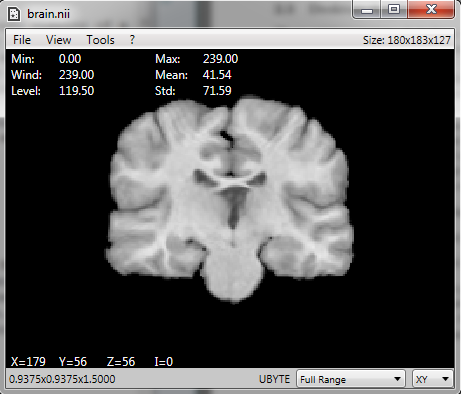
\includegraphics[width=80mm]{graphics/imview_01.png}
\caption{Screenshot of Imview}
\label{fig:UIdesign1}
\end{figure}

\subsubsection{3DSlicer}
3D Slicer is a free open source software that provides a modular platform for image analysis and visualization. Of all the packages, this tool seems to be the most feature rich, which is not surprising as it is funded by a number of American organisations such as  the National Alliance for Medical Image Computing, Neuroimage Analysis Center and others. Although it features a wide variety of tools, the focus will be on the ones relevant to this project. 3D Slicer allows for loading of different files of different formats. It provides options to composite different slices on top of each other for comparison. It supports hardware accelerated volumetric rendering of medical image data. It is widely customisable with global settings. Layouts are also customisable. It has an extensive set of tools for manual and automatic image segmentation. It has an in-built feature to download sample data, which would be a useful inclusion for the web app project. Another powerful feature is that 3D Slicer allows the addition of new functionality and provides a number of generic features not available in competing tools. All in all, 3DSlicer appears like a well designed, user-friendly program that has an overwhelming amount of functionality. It will be another good benchmark and inspiration for this project.

\subsubsection{MIview}
MIview was programmed by Greg Book, is open source and provides much the same functionality as MITK. MIView is an OpenGL based medical image viewer which aims to support a wide range of medical imaging files such DICOM, Nifti, and raster images. It can also read and convert DICOM mosaic images. The main goal of MIView is to provide a platform to load any type of medical image and be able to view and manipulate the image. Volume rendering is also supported. Control-wise, support for mouse-wheel scrolling seems erratic, which makes navigation through the slices more cumbersome. Also the buttons tend to be quite small which also does not improve the user experience. It does not appear to support the loading of multiple files together. A number of predefined color look-up tables are provided.

\subsubsection{Photoshop}
Looking further afield to some graphical editing software programs, some interesting functionality can be discovered. Adobe's Photoshop is well known software for creating and manipulating 2D imagery. When editing an image, the user works with a document. The user can add as many layers as required and edit each layer individually. The layers are composited to form the whole picture. Each layer's opacity and compositing/blending mode can be specified. This could be a worth while to emulate for comparing different medical image files in the web app.

\begin{figure}[ht!]
\centering
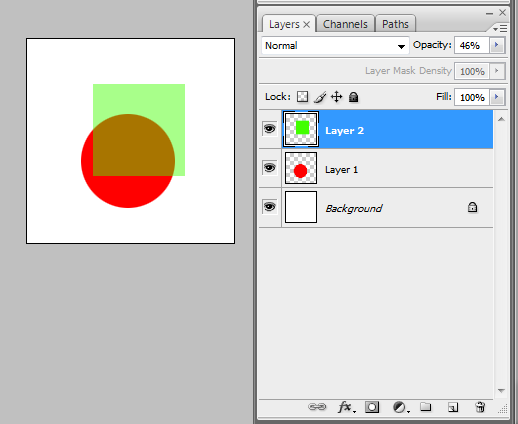
\includegraphics[width=80mm]{graphics/photoshop_01.png}
\caption{Layer compositing in Photoshop}
\label{fig:UIdesign1}
\end{figure}

\subsubsection{Nuke}
The Foundry's Nuke is a compositing package which is used in the Visual Effects Industry to edit and composite 2D images with each other. It is used among others at high profile VFX companies such as Industrial Light and Magic and Weta Digital\cite{nuke1} \cite{nuke2}). The interface differs from Photoshop in that it provides the user with a workplace where any number of nodes can be created. When selecting any node, a graphical display will appear. These nodes can be linked together and do anything from loading a specific image file, transforming the whole node tree or applying an image filter such a film grain. The power of this approach is the modular nature of a tree. Any node can be taken out and reinserted at another place into the tree, thereby changing the final image. Additionally, for comparing different images, by default the software supplies two image buffers which the user can fill with any image of his choice (including of course the result from any node tree in his workspace). Once both buffers are filled, the user can easily toggle between the two images, blend between them by setting the opacity and even use a slider to reveal just a portion of either image. So while Nuke's node-based approach may be overkill for this project, Nuke's image blending seems quite desirable for this project as it would give the user a variety of ways in which he can compare multiple images. 

\begin{figure}[ht!]
\centering
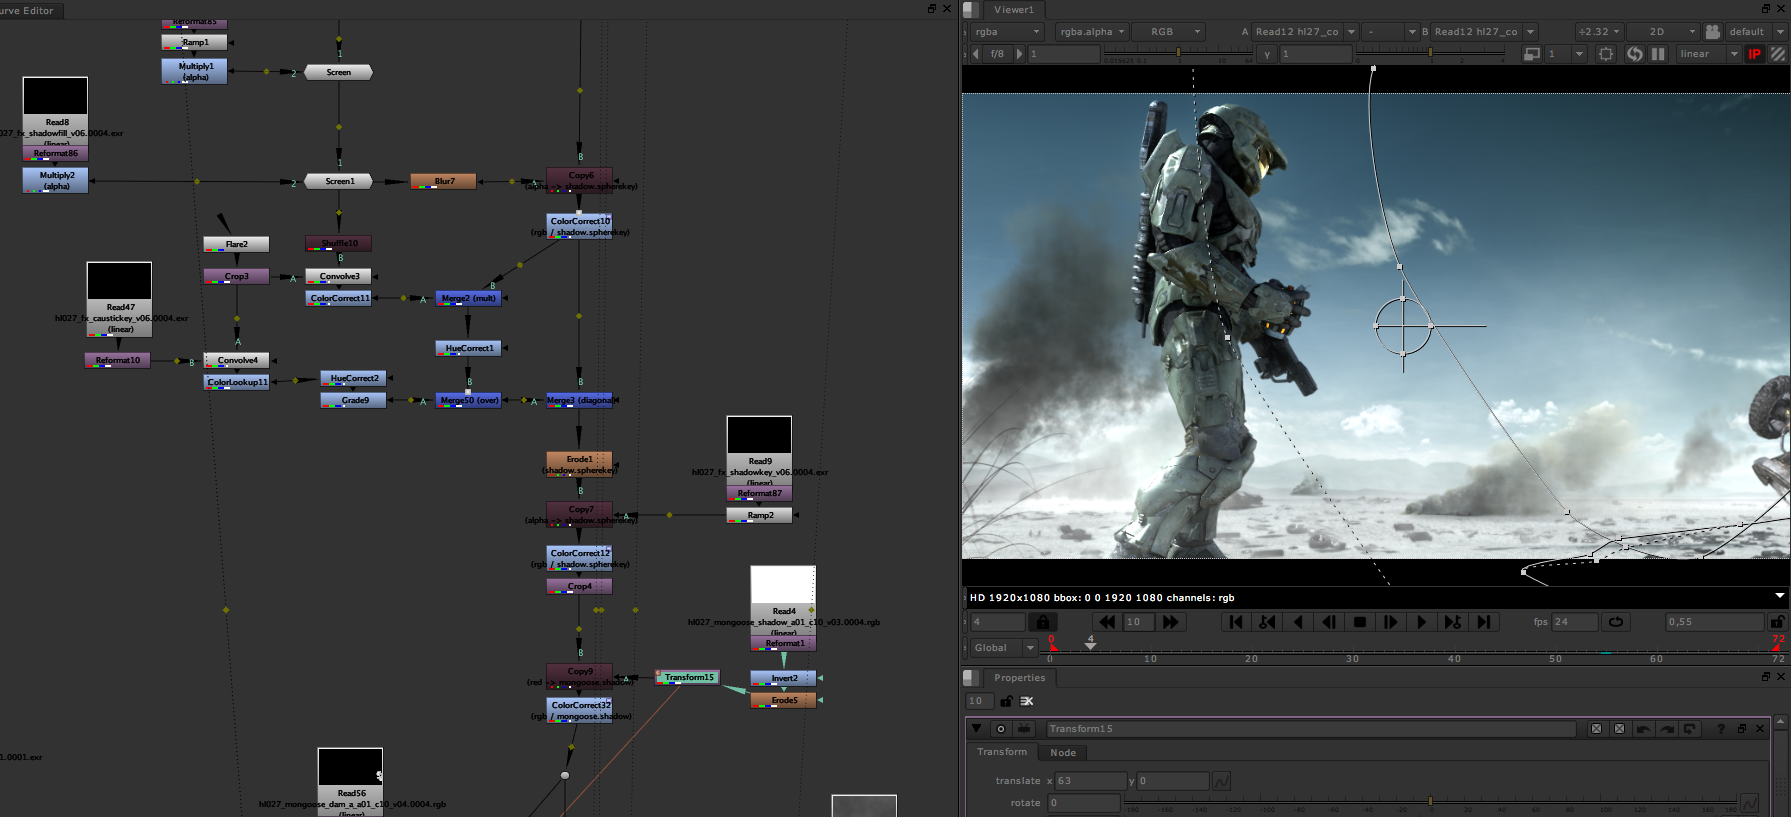
\includegraphics[width=170mm]{graphics/nuke_02.png}
\caption{Nuke's node-based workspace}
\label{fig:UIdesign1}
\end{figure}


\subsection{Interactive Web Graphics}

In order to create an interactive web browser application that provides graphical feedback, the available tools for creating 2D and 3D graphics in a web browser have to be considered. Generally, in the past web browsers have provided several different methods to display 2D and 3D graphics on screen, and only recently with the introduction of HTML5 and WebGL has a widely-conformed standard emerged.

\subsubsection{HTML5}

All websites are grounded by the HTML standard. HTML5 is the latest version of this. It was brought out in this and then and introduced a number of important features that changed how graphics could be communicated via the web. Most importantly it supplied the Canvas element, a scriptable graphical display element and it introduced the WebGL specification, enabling hardware-accelerated 3D Graphics display.


\subsubsection{2D Graphics}

Displaying 2D graphics has long been an integral part of web browsers. Various aspects and methods allow for the generation and manipulation of 2D graphics in a web browser. Aside from simply displaying an image file, there are various other aspects and methods allow for the generation and manipulation of 2D graphics in a web browser

CSS is used to alter an element's style property, but this is not really suitable for creating intricate 2D graphics, as it is typically used to style the look of HTML elements. There are no custom draw commands.

Scalable Vector Graphics (SVG) is like HTML for graphics. It is a markup language for describing all aspects of an image or Web application, from the geometry of shapes, to the styling of text and shapes, to animation, to multimedia presentations including video and audio. It is fully interactive, and includes a scriptable DOM as well as declarative animation (via the SMIL specification). It supports a wide range of visual features such as gradients, opacity, filters, clipping, and masking.
The use of SVG allows fully scalable, smooth, reusable graphics, from simple graphics to enhance HTML pages, to fully interactive chart and data visualization, to games, to standalone high-quality static images. SVG is natively supported by most modern browsers (with plugins to allow its use on all browsers), and is widely available on mobile devices and set-top boxes. All major vector graphics drawing tools import and export SVG, and they can also be generated through client-side or server-side scripting languages.

Finally, the Canvas API is a client-side scripting technology to allow for the rich creation or alteration of raster images (bitmaps) . It uses vector-based programmatic methods to create shapes, gradients, and other graphical effects, and because it has no DOM, it can perform very quickly. Dedicated scripters can develop games or even full-featured applications using the Canvas API, alone or integrated into HTML or SVG. It is supported natively in most modern browsers (with script libraries extending support to all major browsers), and even on some mobile devices.

Before the Canvas API became common place, there were different web browser plug-ins which would display more interactive graphics and videos. Adobe's FlashPlayer and JavaApplets were very common for this purpose. These will be discussed more in detail in the next section, as they were used to display both 2D and 3D graphics.

\subsubsection{3D Graphics}

3D Graphics are usually defined by a space in Cartesian coordinates in which reside three-dimensional objects, as well as a camera object through which the scene is viewed with help of a projection matrix. 3D graphics includes lots of maths with matrices and is computationally much more expensive than drawing 2D graphics. Rendering a scene can mean that the image should be refreshed 60 times a second, which poses a challenge for many browsers.

Broadly speaking, the history of 3D Graphics can be divided into the time before and after the standardisation of WebGL. Before WebGL the standard way to display 3D graphics in a web browser were tied to a browser plug-in that the user would have to download locally to their computer. Adobe's Flashplayer used to be one of the dominant plug-ins. Demonstrating one of the issues with the plug-ins is that they would have to be implemented specifically for each operating system. Furthermore, Apple actually refused to support the format, instead betting on the HTML5 standard. This shows that there are issues with using browser plug-ins, and a more generalised solution was sought for.

Examples JavaApplets, Flash, O3D, 

Microsoft implemented its own plugin Silverlight.

JavaApplets are another alternative, which run on the local machine through the Java virtual machine. However many security issues have been identified with this lately, by some accounts even up to 50\% of all issues.

With the standardisation of HTML5, WebGL and the Canvas element became widely used and supported, and helped to reduce the multitude and clutter of browser-plugins. WebGL is a \textit{JavaScript} API that exposes a computers GPU to the web browser and allows for displaying of complex three dimensional graphics as seen in comparable desktop applications. Although only initially relased in 2011, WebGL is widely supported by most modern browsers (\cite{webGL}), so it's a good time to make use of this for medical visualisation. WebGL is based on OpenGL ES 2.0 and uses the HTML5 canvas element and is accessed using Document Object Model interfaces.

History of WebGL. 

Nowadays, most libraries make use of WebGL and even libraries that used to require a plug-in (example) have now been ported to use WebGL. 
Games in WebGL



\subsection{Web Framework XTK}

As suggested in the project specification, the goal of this project is to use the \textit{X Toolkit}(\textit{XTK}), a \textit{JavaScript}-based framework for visualizing and interacting with medical imaging data using \textit{WebGL}. It was developed and maintained by Haehn et al of the Fetal-Neonatal Neuroimaging and Developmental Science Center at Childrens Hospital Boston, Harvard Medical School, US (\cite{xtk}). \textit{XTK} provides an API to load medical images, based on \textit{WebGL} technology for displaying 3D graphics and the \textit{HTML5} canvas elements to display 2D components. It hides a lot of the low-level elements of \textit{WebGL} and is designed to load and configure medical image data files of various types (including NIfti). The library is well documented and comes with several tutorials as well as a number of example applications, which will be discussed in the next section. It appears to follow closely the suggestions laid out in section 2.1 (Medical Imaging) in that it provides means to display 2D and 3D slice visualisations (Surface Shaded Display and Volume Rendering are supported), with simple mouse-based controls. It allows for loading of label (segmentation) maps which can overlaid on top of the image data files. It also features color tables (LUTs) to display the data.

The \textit{XTK} library also provides a module for creating User Interface (UI), that can be overlaid on top of the image viewers, with easy controls to connect the image content with the UI controls.
The popular forum for coding questions Stackoverflow hosts about 100 questions regarding \textit{XTK} to date, and occasionally the \textit{XTK} developers offer up answers.


\subsection{Web Applications}

\subsubsection{SliceDrop}
The \textit{XTK} library also provides links to example applications. One of these is \textit{SliceDrop}\cite{slicedrop} which has written by the \textit{XTK} developers and appears to be a testing bed for many of \textit{XTK}'s features as it is often referred to on the \textit{XTK} Stackoverflow forums. It provides part of the desired functionality and shows off the possibilities provided by \textit{XTK}, but also outlines some of its short comings. Like the desktop software \textit{MITK}, the user can load a file and view it in the standard 4 views, split into 3D and 2D windows. The layout of these views is somewhat customisable, although not to the extent of the \textit{MITK}. The user can interact with the images by scrolling the mouse wheel, which changes the index of the current slice. An interesting feature which has been added lately is the incorporation of popular file sharing site \textit{DropBox} to allow users to share files more easily across the internet.

There appear to be some bugs in \textit{SliceDrop}. When loading \textit{NRRD} files, as the image is offset and not centered. The image brightness controls seem not calibrated correctly, as with little mouse interaction, the brightness will clamp to white or black and can not be reset other than restarting the program (refreshing the page for web-apps). Furthermore the app does not allow to load custom labelmaps. Also the viewers provide some functionality which is not clearly communicated to the user, such as holding the 'shift' button and move the mouse will adjust the slice index of the other viewers. In general \textit{SliceDrop} has less than the minimum functionality required for this project, but shows the potential of the \textit{XTK} library. 


\subsection{Brainbook}
\textit{Brainbook}\cite{brainbook} is a web-app which builds on and extends the features of \textit{SliceDrop} by adding painting tools. It allows the user to paint onto a given file with a standard brush a number of auto selection tools which will fill out a region in 2D or 3D space. The web app offers to save the file, but at time of writing this feature was not working correctly. Since heavily based on \textit{SliceDrop}, it features similar advantages and disadvantages, but provides the painting functionality that is desirable for this project. Therefore it should be of benefit to study this implementation.

\subsection{DWV - DICOM Web Viewer}
This viewer does not provide much functionality other than scrolling through one stack of slices. The user interface is sparse and does not give sufficient feedback to the use of what is currently happening. It uses the HTML5 Canvas element to display the file contents.

\begin{figure}[ht!]
\centering
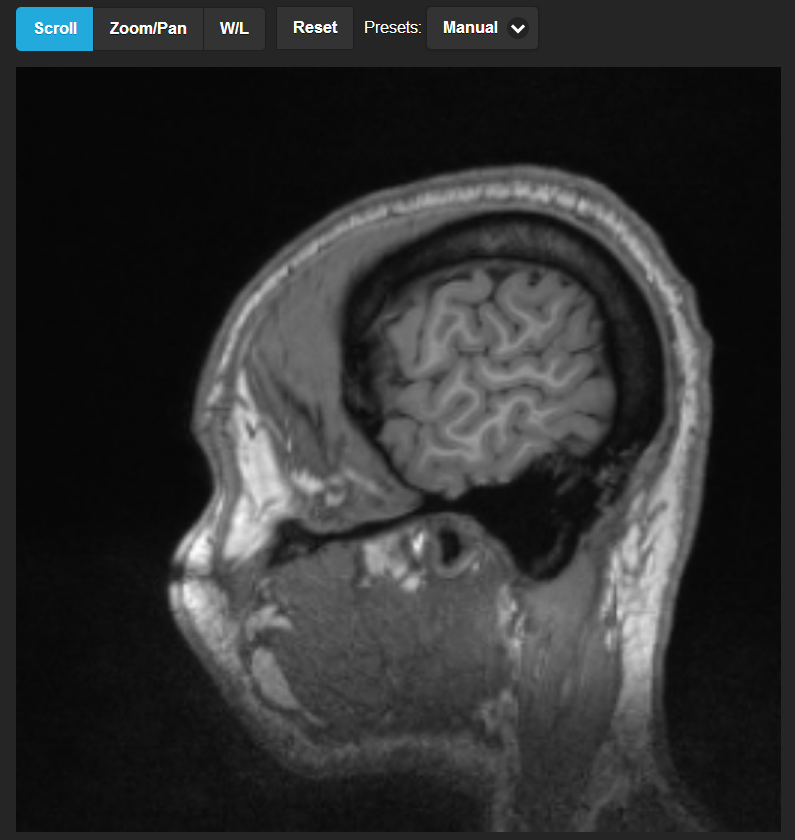
\includegraphics[width=100mm]{graphics/webViewer_01.png}
\caption{DWV User Interface}
\label{fig:UIdesign1}
\end{figure}

\subsection{Papaya}
Papaya\cite{papaya} is a \textit{JavaScript}-based medical image viewer with limited functionality. It has a clean uncluttered design, is easy to use and gives good visual feedback to the user. It successfully adheres to the user control guidelines outlined in section 2.1. It only displays 2D views of slices and does not allow any customisation in terms of label maps, windowing or compositing. It also uses the HTML5 Canvas element to render the 2D data.

\begin{figure}[ht!]
\centering
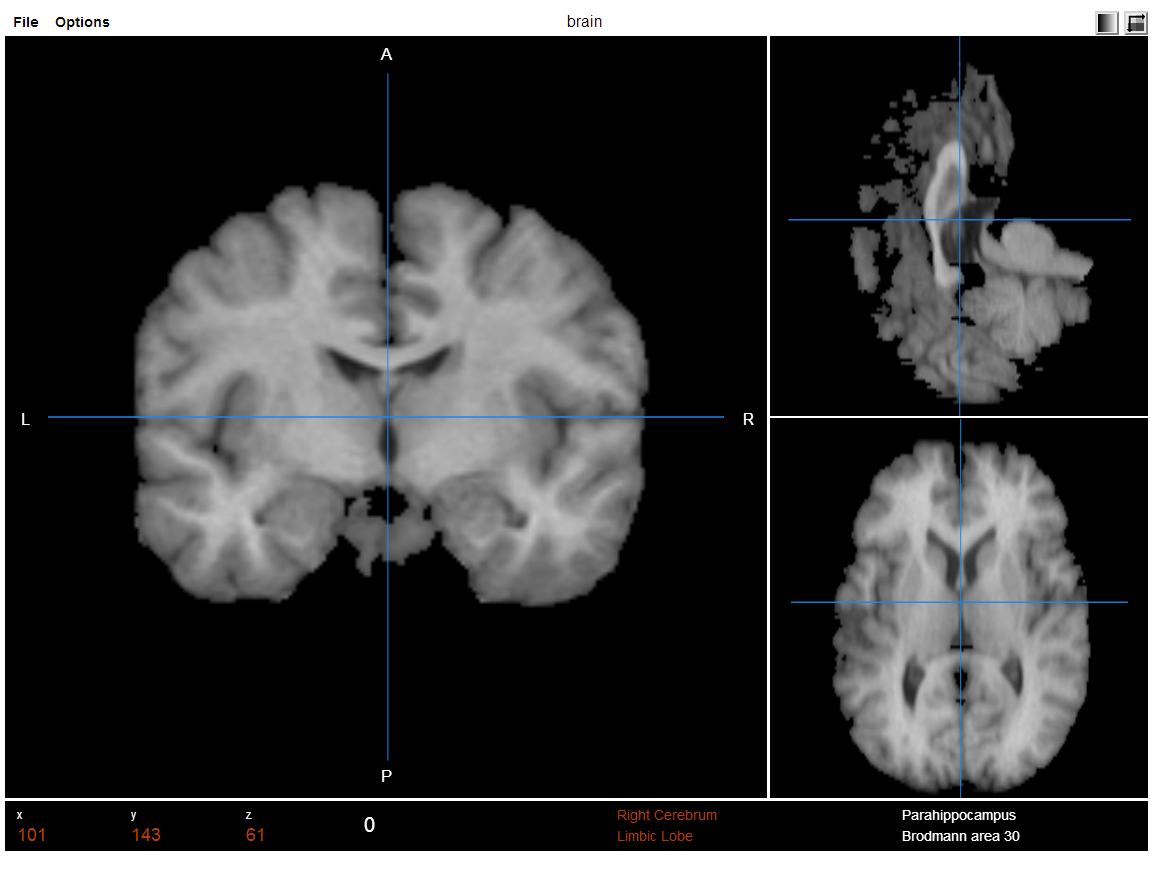
\includegraphics[width=100mm]{graphics/webViewer_02.png}
\caption{Papaya Interface}
\label{fig:UIdesign1}
\end{figure}

\subsection{Other}

The website \url{http://www.idoimaging.com} lists a number of other available browser-based viewers.


\subsection{Web Frameworks for Single Page Apps}

Programming for modern webpages which require more complex behaviour than just displaying information can get quite involved. Generally it takes at least HTML, CSS and \textit{JavaScript} to create a useful website. It is possible to include the code from each language in the main index.html file, but this is undesirable as it lacks modularity and will be hard to test and debug.

At the time of writing, \textit{Backbone} seems to be a good choice to manage the complexity and structure of the project. \textit{Backbone} is used to structure client-side applications (those that run in a web browser). It was written by Jeremy Ashkenas and is designed for developing single-page web applications, and for keeping various parts of web applications synchronized. It is based on the model–view–presenter (MVP) application design paradigm, providing Events, Models, Collections and Views. Models represent the information in class-like structures, Collections are lists of Models and Views handle the visual representation on the actual HTML site. Finally Events are used to keep track of state changes across the website elements, models and views. It builds on \textit{jQuery} and Underscore.js, both libraries which simplify dealing with HTML elements. It also provides inheritance for its models, collections and views.

Regarding the design aspect, it looks like twitter-bootstrap.js supplies a convenient library for creating visually pleasing user interface elements. This will cut down on having to spend time to design custom elements with CSS and \textit{JavaScript}. Bootstrap.js supplies buttons, drop-down menus and commonly-used icons. Some specific UI control elements are not provided by Bootstrap, so \textit{jQueryUI} will be used. It enables the creation and customisation of complex elements such as slider elements with multiple slider tabs, which will allow for a better user experience. Also, it's dependent on the \textit{jQuery} library which is already being used for \textit{Backbone}.

As this project will make of several modules, it will be important to manage the dependencies of the modules. For example Underscore.js and \textit{jQuery} will need to load before \textit{Backbone.js} is used. \textit{XTK} and twitter-boostrap are additional modules that will have to be loaded. \textit{RequireJs} is a \textit{JavaScript} library that provide the ability to asynchronously load nested dependencies. Traditionally \textit{JavaScript} files or modules are loaded sequentially, where the order matters in case a module depends on another module. Additionally it will be helpful to manage the different HTML templates required for the various elements of the web app. \textit{RequireJs} will make it possible to split up everything into neat modules and templates and facilitate testing of all the components.




\section{Requirements}

The goal of this project is to build a web browser based Medical Image Viewer. This will be achieved by making use of WebGL to display 2D and 3D graphics. In general the project aims to provide similar functionality and user experience as the desktop application MITK (discussed earlier). The essential requirements are as follows:

\begin{itemize}
\item The user can load and view a scan file (of type NIfTI)
\item The user can view a file in 2D and 3D
\item The user can easily navigate through the 2D and 3D viewers, with emphasis on intuitive user experience
\item The web-app provides controls for viewing the scan files at different brightness and contrast levels
\item The user can load and view a labelmap for a given scan file
\item The user can load additional scan or label maps into the viewer and compare them to previously loaded files with a set of intuitive controls
\item Provide different color-lookups (for label-maps, heat maps)
\item Provide sample data to use if user has no files of his own
\end{itemize}

Given enough time, secondary requirements can be implemented, which are considered to be more complicated:

\begin{itemize}
\item The user can paint a custom labelmap for a given scan file with a set of intuitive tools. The primary goal will be that the user can paint areas manually on individual slices. Provided there is enough time, some semi-automatic painting tools will also be implemented that will allow the user to specify regions in the 3D space with automatic selection tools. 
\item The user can save a labelmap to his computer
\item The user can create and save custom annotation maps to label given scans
\item The web app provides a method for sharing  means of sharing data across the internet (similar to the DropBox implementation in SliceDrop)
\item The web app provides image filters that can be applied to a scan or label map
\item The web app provides measuring tools that can be applied to a scan or label map
\item A three dimensional, parameterised model of the scan be viewed in the 3D view
\item The 'cine mode' feature allows for an animation along a specified axis
\end{itemize}

\section{Use Cases}

A small selection of use cases have been discussed with the project supervisor. The following were suggested:

\begin{itemize}

\item A user loads two medical images files from a patient that has undergone brain surgery. The user wants to compare the scans from before the operation to afterwards. The user needs to be able to compare the two files in meaningful ways, with tools for image comparison and compositing.

\item A user wants to create a custom label map by highlighting a certain section of a loaded scan. The user can use provided paint tools to paint individually on each slice, or alternatively use semi-automatic tools like filling in regions within a given color range to speed up this process. The user can save out this custom label map in NIfTi format.

\item The user wants to create annotations for a file. He can use the software to create annotated planar or cuboid regions to for example specify where a given organ is in the scan. The software provides intuitive controls and helpful visual feedback to facilitate this process. The user can save out this files as a custom data file.

\item A user wants to communicate with another user who is not present in the same location. The first user can use the software to provide links to specified medical image files to the second user. The second user can load these files with the software for analysis.

\end{itemize}

\section{Progress}

Some effort has already gone into planning and implementing the project. The initial plan was to create a working prototype in a relatively short time. This was however foiled by the complexity of the task of creating a functioning web-app. At first, tests were done building on tutorials that are provided by the \textit{XTK} toolkit site. This included a simple HTML front end as well as some \textit{JavaScript} files to handle the \textit{XTK} objects.

Loading local files in a web browser proved to be one of the early issues. Due to security issues, Chrome and other browsers do not allow local files to be loaded onto the HTML canvas element, tying into the same origin policy that browsers try to uphold. A way around this was found by analysing the SliceDrop code and noticing that it uses the HTML FileReader to convert the local file into a byteArray which can then be loaded into the \textit{XTK} viewers.

Having some concerns that modifications will have to be made to the \textit{XTK} toolkit, the author managed to successfully clone and fork the project from github. Since things are never as easy as hoped for, editing and rebuilding the toolkit proved tricky, since it employs yet another unknown \textit{JavaScript} library, called GoogleClosure.js. After learning how to use this module and other little issues mainly due \textit{XTK} being developed on Linux and not Windows, the OS the project is currently being developed on, the toolkit managed to recompile successfully.

Once some basic tests with the \textit{XTK} toolkit proved that it could be used to display local scan files, it was time to start adding some functionality to the website. This quickly showed that the previous implementation of the HTML website was highly naive, and that it would require a restructuring from the ground up. Almost as an example of why web programming can be tricky, the HTML site was mixing elements from HTML, CSS and \textit{JavaScript} without much structure. When separating out the \textit{JavaScript} parts into separate files, the issue of module loading and dependency became apparent.

From the group project earlier in the term, the author was aware of \textit{JavaScript} libraries that aid in structuring a web-app such as \textit{Backbone.js}, \textit{RequireJs} and \textit{jQuery}. So the next few days were spent trying to get to grips with these and understanding generally how web apps are built. This seems to be a rich topic in its own right, and will undoubtedly take more time still to become comfortable with. However it helps that \textit{Backbone} tends to enforce a somewhat object-oriented structure, which ties development back to principles learned in the Masters course over the year. Even when starting to implement the \textit{Backbone} it becomes apparent how easy it is to fall back into mixing different language in the files and to enforce that every component just does the one task it is supposed to do. Talk about templates...

When realising that an object-orientated structure can and should be applied to the project, it prompted the author to create a UML diagram with possible class design (see Appendix). This will prove useful when implementing the \textit{Backbone} components and helps to visualise the flow of control of the web-app. Additionally, visual UI design have been made to show how the front-end would look like to the user and what controls would available to him or her (see Appendix). After it some research it also became apparent that yet another \textit{JavaScript} library called twitter-bootstrap is very popular among the web community to create UI designs for buttons and menus, so time was spent learning how to tie this into the project.
Currently, the plan is still to create a working prototype that has all the essential requirements fulfilled.


\subsection{Concerns}

\subsubsection{XTK}

So far, testing the \textit{XTK} toolkit has revealed some concerns. In general the library is not as modularised as hoped for, as it does not seem possible to add a custom number of label maps. There is at present also no way to paint a custom label map. However, as already discussed, it is possible to fork the project from github and introduce changes, so this will have to be explored when adding additional features.

Other useful functionality is hard-coded into the library, which may need suppressing or changing of the input triggers. For example currently, the are no display lines for all viewers when one clicks or moves the mouse over one view. Furthermore the user has to hold down the shift key and move the mouse over a view, to affect the slice indices of the other views. This can hopefully be tweaked in the module.

Some design decisions in the \textit{XTK} library are so far not ideal. For example when loading a file into a \textit{XTK} volume, (which is then attached to a \textit{XTK} renderer), the actual loading of the file happens only once the first \textit{XTK} renderer has its render() function called. In the case of having multiple \textit{XTK} renderers initiated(as the standard 3D/X/Y/Z format), the other renderers have to wait until the loading is complete and can only afterwards call their render() function. If calling render before the loading is complete, according to the \textit{XTK} developers, the internal object data can get corrupted. For the scope of this project, this is not ideal as it implies that further management is required.

There also appears to be a bug with loading NRRD files, as they as displayed with an offset in the 2D and 3D viewers. This behaviour is visible in SliceDrop as well as in the \textit{XTK} tutorials. The \textit{XTK} developers have been made aware of the problem.

It appears that there is only a very small and inactive community for the \textit{XTK} library. There is a group on the popular tech forum StackOverflow but questions are being asked infrequently and get answered even more rarely.

One strategy to follow will be to use the \textit{XTK} renderers solely for their image generation and override all the UI functionality. This could be achieved by creating a custom renderer class that simply copies the imageData from the \textit{XTK} renderers. The HTML5 canvas element provides functionality for this, but will have to be tested for speed drawbacks. It would seem that this method would bring along a multitude of advantages, such as easily creating custom text and graphic overlays, blending between different renderers and hiding the more obscure features of the \textit{XTK} loading process as discussed earlier in this section, all without having to rewrite the \textit{XTK} library itself. A drawback would be that a lot of UI interaction methods would have to be rewritten (such as middle-mousing over canvas changing the index, etc), but one would also have a lot more control in redesigning the user experience.

\subsubsection{Cross Browser Compatibility}

Judging from limited previous experience, cross browser compatibility can be a difficult issue, as different browsers on different operating systems are implemented differently. Therefore what might work very well on Chrome could not work at all on Internet Explorer, as some functions are implemented differently or not even available in certain browsers. Therefore the app will have to be tested thoroughly across a variety of web browsers and operating systems.


\newpage

  \begin{thebibliography}{1}

  \bibitem{book} Bernhard Preim, Charl Botha, {\em Visual Computing for Medicine} Second edition. 2014
  
   \bibitem{xtk} {\em Xtk Toolkit } \url{https://github.com/xtk/X#readme}
   
     \bibitem{nifti1} {\em NIfTI-1 Data Format} \url{http://nifti.nimh.nih.gov/nifti-1}
     
	\bibitem{nifti2} {\em The NIFTI file format} \url{http://brainder.org/2012/09/23/the-nifti-file-format/} 
   
      \bibitem{backbone} {\em Neuroimaging in the Browser using the X Toolkit } \url{http://www.frontiersin.org/10.3389/conf.fninf.2014.08.00101/event_abstract} 

  \bibitem{backbone} {\em BackboneJs } \url{http://backbonejs.org} 
  
  \bibitem{require} {\em RequireJs } \url{http://requirejs.org} 
  
  \bibitem{bootstrap} {\em Twitter-Bootstrap } \url{http://getbootstrap.com} 	
  
  \bibitem{w3graphics} {\em W3 - Graphics } \url{http://www.w3.org/standards/webdesign/graphics}
  
  \bibitem{brainbook} {\em Brainbook } \url{http://users.loni.ucla.edu/~pipeline/pain} 
  
  \bibitem{papaya} {\em Papaya } \url{http://ric.uthscsa.edu/mango/papaya.html} 
  
    \bibitem{dvw} {\em Dwv DICOM Web Viewer. } \url{http://ivmartel.github.io/dwv} 

    \bibitem{slicedrop} {\em Slice:Drop} \url{http://slicedrop.com} 
    
  
    
  \bibitem{nuke1} {\em Weta Digital Purchases Site License Of Nuke } \url{http://www.fxguide.com/quicktakes/weta-digital-purchases-site-license-of-nuke} 
        
  \bibitem{nuke2} {\em Industrial Light \& Magic Purchases Nuke Site Licence } \url{http://www.creativeplanetnetwork.com/the_wire/2009/06/09/industrial-light-magic-ilm-purchases-nuke-site-licence} 

    \bibitem{3Doverview} Alun Evans, Marco Romeo, Arash Bahrehmand, Javi Agenjo, Josep Blat, {\em 3D graphics on the web: A survey } \url{http://www.sciencedirect.com/science/article/pii/S0097849314000260}. Interactive Technologies Group, Universitat Pompeu Fabra, Barcelona, Spain


  \end{thebibliography}

\newpage

\section{Appendix}


\begin{figure}[ht!]
\centering
\includegraphics[width=170mm]{../../Design/UML_design_01.jpg}
\caption{Early UML design}
\label{fig:UIdesign1}
\end{figure}


\begin{figure}[ht]
  \begin{adjustbox}{addcode={\begin{minipage}{\width}}{\caption{%
     Early UI design
      }\end{minipage}},rotate=90,center}
      \includegraphics[scale=.45]{../../Design/UI_design_02.jpg}%
  \end{adjustbox}
\end{figure}


\end{document}
